\chapter{Modélisation du comportement statique des systèmes}
\thispagestyle{plain} % Supprimer le header & le footer sur cette page en laissant la numérotation
\newpage

%----------------------------------------------------------------------------------------
%	Frottements
%----------------------------------------------------------------------------------------

\section{Frottements \& Arc-boutement}

\exercice{Parallépipède sur plan incliné}
\texttt{Rappel sur les lois de coulomb (contact surfacique)}

Soit un parallélépipède $1$ (de masse $m$ et de centre de gravité $G$) posé
sur un plan incliné $0$.

\begin{center}
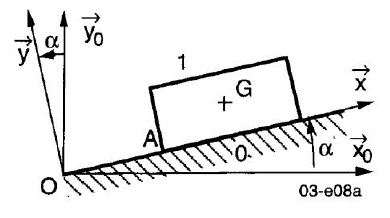
\includegraphics[scale=0.7]{png/plan_incline.png}
\end{center}

On pose $\alpha=(\overrightarrow{x_0},\overrightarrow{x})$, $\overrightarrow{AG}=a.\overrightarrow{x}+b.\overrightarrow{y}$.\\
Le coefficient d’adhérence entre les $2$ solides est noté $\mu$ et le problème est supposé plan.

\subsubsection{Travail demandé}
\begin{enumerate}
\item Déterminer $T_{0\rightarrow1}$, l'action mécanique de $0$ sur $1$ en $G$.
\begin{itemize}
\item d’abord si on suppose la liaison parfaite et que le problème n’est pas plan,
\item puis si on suppose la liaison parfaite et que le problème est plan,
\item enfin si on suppose la liaison avec adhérence et que le problème est plan (modèle pour la
suite de l’exercice).
\end{itemize}
\item Appliquer le PFS sur $1$ et en déduire la condition sur $\alpha$ pour qu’il n’y ait pas de glissement.
\item Déterminer le moment en $A$ de la pesanteur sur $1$ et en déduire la condition sur $\alpha$ pour qu’il n’y ait pas de basculement du solide $1$ ?
\item En déduire la condition pour que le basculement se fasse avant le glissement (lorsque l'on augmente $\alpha$).
\end{enumerate}


\newpage

%--------------------------------------------

\exercice{Embrayage à friction monodisque de véhicules automobiles}

On modélise l'embrayage par deux disques creux identiques ($1$ et $2$) en contact grâce à une action axiale $\overrightarrow{F_a}$.\\
Le rayon intérieur des deux disques vaut : $R_{min}$. Le rayon extérieur des deux disques vaut : $R_{max}$. On donne $\mu$ le coefficient d’adhérence entre
les deux pièces.

\begin{center}
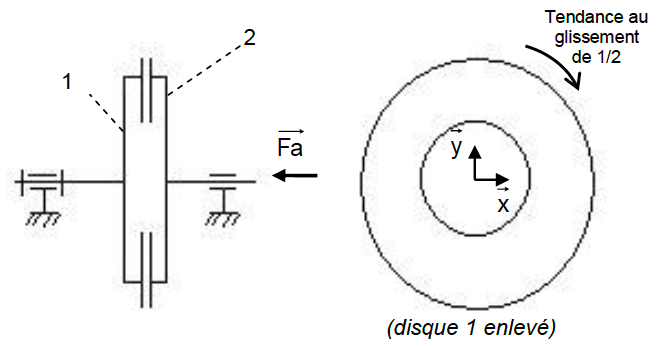
\includegraphics[scale=0.5]{png/embrayage.png}
\end{center}

\subsubsection{Travail demandé}
\begin{enumerate}
\item Refaire en grand les deux schémas ci-dessus : un dans le plan $(y, z)$ et l’autre dans le plan $(x, y)$, en plaçant les actions élémentaires normale et tangentielle de $2$ sur $1$ en un point $Q$ quelconque de la surface de contact.
\item Exprimer $\overrightarrow{dF_{2\rightarrow1}(Q)}$.
\item Déterminer le couple maximal transmissible en fonction de $p$ (la pression exercée sur les disques creux) et des caractéristiques géométriques de l’embrayage.
\item Déterminer l’action axiale $\overrightarrow{F_a}$ (qui crée les $\overrightarrow{dN}$ ) en fonction de $p$ et des caractéristiques géométriques de l’embrayage.
\item En déduire le couple maximal transmissible en fonction de $\overrightarrow{F_a}$ (et non en fonction de $p$) et des caractéristiques géométriques de l’embrayage.
\end{enumerate}

\newpage

%--------------------------------------------

\exercice{Embrayage conique des synchroniseurs de boîte de vitesses}

On modélise le pignon fou et l'anneau de synchronisation par deux cônes en contact grâce à une action axiale $\overrightarrow{F_a}$.\\
Le rayon intérieur des deux cônes vaut : $R_{min}$. Le rayon extérieur des deux cônes vaut : $R_{max}$. Le demi-angle au sommet des deux cônes vaut : $\alpha$. On donne $\mu$ le coefficient d'adhérence entre
les deux pièces.

\begin{center}
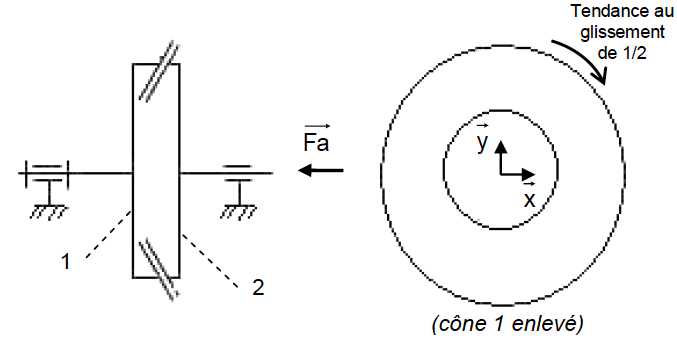
\includegraphics[scale=0.5]{png/embrayage2.png}
\end{center}

\subsubsection{Travail demandé}
\begin{enumerate}
\item Refaire en grand les deux schémas ci-dessus : un dans le plan $(y, z)$ et l’autre dans le plan $(x, y)$, en plaçant les actions élémentaires normale et tangentielle de $2$ sur $1$ en un point $Q$ quelconque de la surface de contact.
\item Exprimer $\overrightarrow{dF_{2\rightarrow1}(Q)}$.
\item Déterminer le couple maximal transmissible en fonction de $p$ (la pression exercée sur les disques creux) et des caractéristiques géométriques de l’embrayage.
\item Déterminer l’action axiale $\overrightarrow{F_a}$ (qui crée les $\overrightarrow{dN}$ ) en fonction de $p$ et des caractéristiques géométriques de l’embrayage.
\item En déduire le couple maximal transmissible en fonction de $F_a$ (et non en fonction de $p$) et des caractéristiques géométriques de l'embrayage.
\end{enumerate}

\correction{
\begin{enumerate}
\item Schéma corrigé
\begin{center}
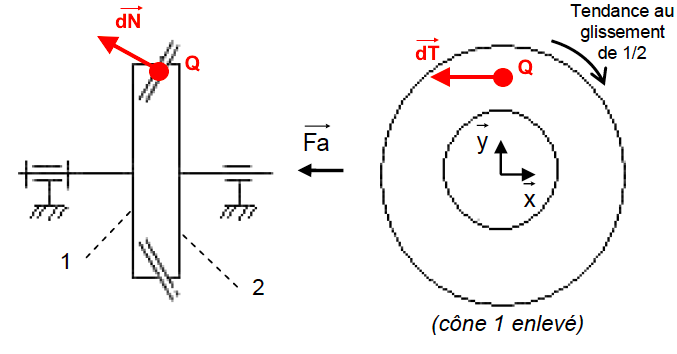
\includegraphics[scale=0.5]{png/embrayage2_correction.png}
\end{center}

\item $\boxed{\overrightarrow{dF_{2\rightarrow1}(Q)}=\overrightarrow{dN}+\overrightarrow{dT}}$ avec $\overrightarrow{dT}=\mu\overrightarrow{dN}$

\item $dC = rdT = r\mu dN$ avec $dN = pdS$ et $dS = rd\theta dl = \frac{rd\theta dr}{\sin\alpha}$\\
d'où après intégration $\boxed{C=\frac{2\pi \mu p}{3\sin\alpha}\left( R_{max}^3-R_{min}^3\right)}$

\item Comme $dF_a = dN \sin\alpha$ on en déduit $\boxed{F_a=p\pi\left( R_{max}^2-R_{min}^2\right)}$

\item Ainsi $\boxed{C=\frac{2\mu F_a}{3\sin\alpha}\frac{R_{max}^3-R_{min}^3}{R_{max}^2-R_{min}^2}}$
\end{enumerate}
}
\newpage

%--------------------------------------------

\exercice{Porte tôle}

Un porte tôle est représenté ci-dessous. Les molettes ont une liaison pivot d'axe $(B,\overrightarrow{z})$ et $(B',\overrightarrow{z})$ avec le flasque. Elles serrent la tôle sous l'action mécanique de deux biellettes articulées en $C$ et $C'$ avec les molettes et en $D$ et $D'$ avec l'étrier auquel est accroché le câble.\\
On suppose que toutes les liaisons sont sans frottement, sauf bien sûr la liaison entre la tôle et les molettes, et que toutes les pièces sont de masse négligeable devant la masse de la tôle.\\
On donne (en millimètres)
\begin{center}
$\left\{
\begin{array}{rcl}
	\overrightarrow{IA}=-30.\overrightarrow{y}\\
	\overrightarrow{IC}=-\overrightarrow{IB}=15.\overrightarrow{x}+12.\overrightarrow{y}\\
	\overrightarrow{ID}=102.\overrightarrow{x}-10.\overrightarrow{y}
\end{array}\right.$
\end{center}

\begin{center}
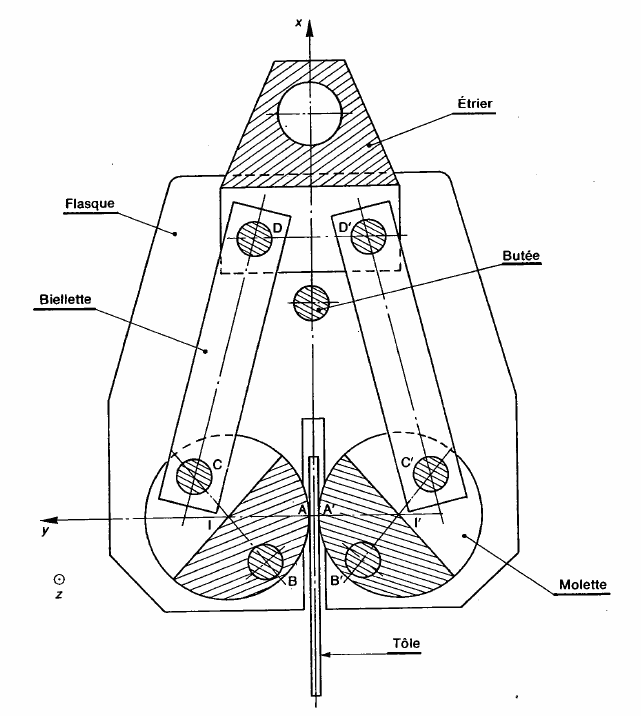
\includegraphics[scale=0.5]{png/molettes.png}
\end{center}

\subsubsection{Travail demandé}
Déterminer la valeur minimale du coefficient de frottement entre la tôle et les molettes pour que le mécanisme puisse fonctionner.


\newpage

%--------------------------------------------

%\exercice{Variateur à courroie}
%
%\begin{center}
%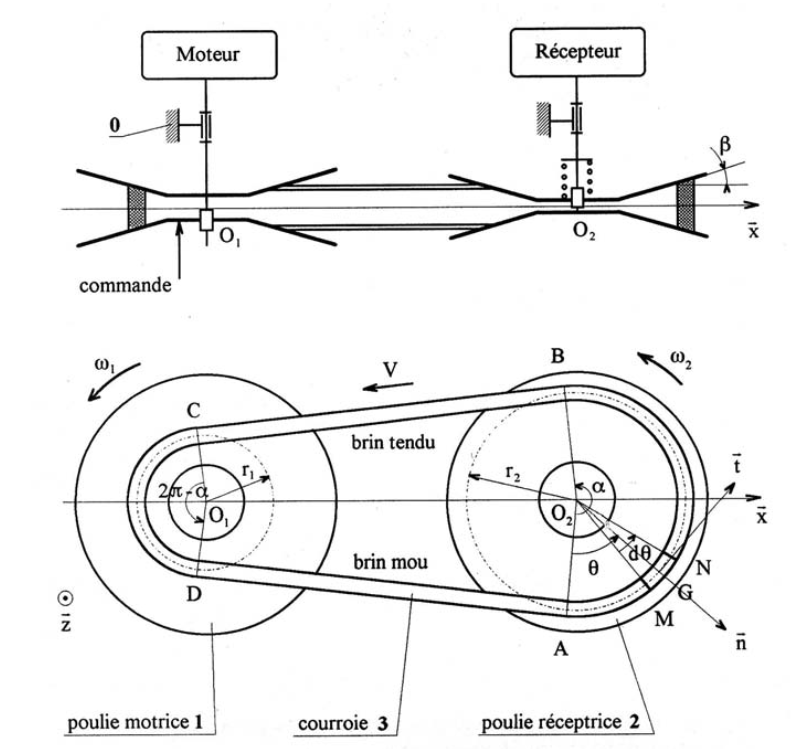
\includegraphics[scale=0.4]{png/courroie1.png}
%\end{center}
%
%Un variateur permet la transmission de puissance d'un arbre moteur vers un arbre récepteur en faisant varier le rapport de réduction de la vitesse de manière continue entre deux limites. Le variateur étudié comporte une poulie motrice $1$, une poulie réceptrice $2$ et une courroie à section trapézoïdale transmettant la fréquence de rotation. La variation de la vitesse s'obtient en réglant l'écartement des flasques des poulies, faisant ainsi varier les diamètres d'enroulement de la courroie.
%
%\begin{center}
%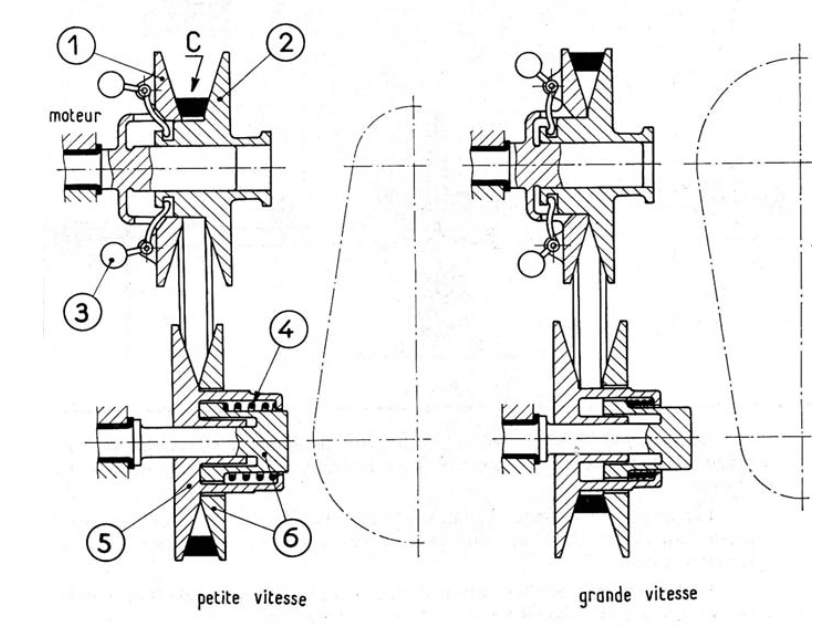
\includegraphics[scale=0.4]{png/courroie2.png}
%\end{center}
%
%Le repère $R(O_1,\overrightarrow{x},\overrightarrow{y},\overrightarrow{z})$ est lié au bâti $0$ du mécanisme. Le plan de symétrie des poulies et de la courroie est parallèle au plan $(O_1,\overrightarrow{x},\overrightarrow{y})$.\\
%La \textbf{poulie $1$} est en liaison pivot parfaite d'axe $(O_1,\overrightarrow{z})$ avec le bâti $0$. On pose $\Omega(1/0) = \omega_1.\overrightarrow{z}$ avec $\omega_1 > 0$. L'action mécanique de l'actionneur sur l'arbre de la poulie $1$
%se modélise par :\\
%$T_{m\rightarrow1} = \left\{
%\begin{array}{rcl}
%	0 \\
%	C_1.\overrightarrow{z}
%\end{array}\right.$ avec $C_1 > 0$\\
%La \textbf{poulie $2$} est en liaison pivot parfaite d'axe $(O_2,\overrightarrow{z})$ avec le bâti $0$. On pose $\Omega(2/0) = \omega_2.\overrightarrow{z}$ avec $\omega_2 > 0$. L'action mécanique de l'actionneur sur l'arbre de la poulie $2$
%se modélise par :\\
%$T_{r\rightarrow2} = \left\{
%\begin{array}{rcl}
%	0 \\
%	-C_2.\overrightarrow{z}
%\end{array}\right.$ avec $C_2 > 0$\\
%????
%%La \textbf{courroie $3$} de section trapézoïdale, inextensible, de masse linéique $\rho$, possède des rayons moyens d'enroulement respectifs sur la poulie $1$, $r_1$ et la poulie $2$, $r_2$. On suppose qu'il n'y a pas de glissement entre la courroie et les poulies. Les angles d'enroulement sont respectivement $\widehat{CO_1D} = 2.\pi − \alpha$, sur $1$ et $\widehat{AO_2B} = \alpha$ sur $2$.\\
%%L'inclinaison des flancs des flasques des poulies est notée $\beta$ et le facteur de frottement entre une poulie et la courroie est noté $f$.
%
%
%\correction{ 
%}
%\newpage

%--------------------------------------------

\exercice{Arc-boutement}
Sur une tige $0$ de rayon $r$ peut glisser un coulisseau $1$ en équerre dont la longueur de la portée (contact sur la tige) est $2h$. La masse du coulisseau est notée $m$ et son centre d'inertie $G$.

\begin{center}
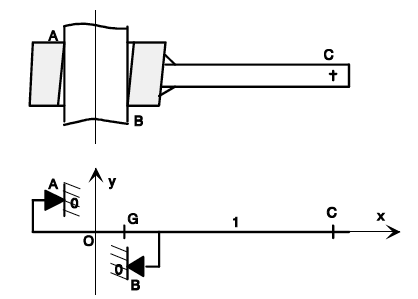
\includegraphics[scale=0.5]{png/arcbout.png}
\end{center}

\subsubsection{Données}
Au point $C$ on applique une force $\overrightarrow{F}=-F\overrightarrow{y}$\\
$\overrightarrow{OA}=-r\overrightarrow{x}+h\overrightarrow{y}$\\
$\overrightarrow{OB}=r\overrightarrow{x}-h\overrightarrow{y}$\\
$\overrightarrow{OG}=d\overrightarrow{x}$\\
$\overrightarrow{OC}=c\overrightarrow{x}$

\subsubsection{Travail demandé}
\textbf{\textit{Partie A :}} On considère que le contact est parfait au point $A$ et qu'il existe un facteur de frottement $f=\tan(\phi)$ au point de contact $B$.
\begin{enumerate}
\item Modéliser (modélisation plane) toutes les actions mécaniques appliquées au solide $1$. On fera l'hypothèse qu'il n'y a pas de glissement en $B$.
\item Déterminer les actions mécaniques de la tige sur le coulisseau.
\item Donner la condition impliquée par l'hypothèse faite à la question $1$.
\item Donner la condition la condition sur $c$, $r$, $h$ et $f$ pour qu'il y est arc-boutement. Il y a arc-boutement si la pièce $1$ ne glisse pas lorsque $F$ devient très grand. ($F>>mg$)
\item Retrouver le résultat de la question $4$ graphiquement.
\end{enumerate}
\textbf{\textit{Partie B :}} Reprendre l'exercice en considérant qu'il existe un facteur de frottement $f=\tan(\phi)$ (non nul) aux deux points de contact $A$ et $B$.

\newpage

%----------------------------------------------------------------------------------------
%	Statique graphique
%----------------------------------------------------------------------------------------

\section{Statique graphique}

\exercice{Grue de port}

\begin{center}
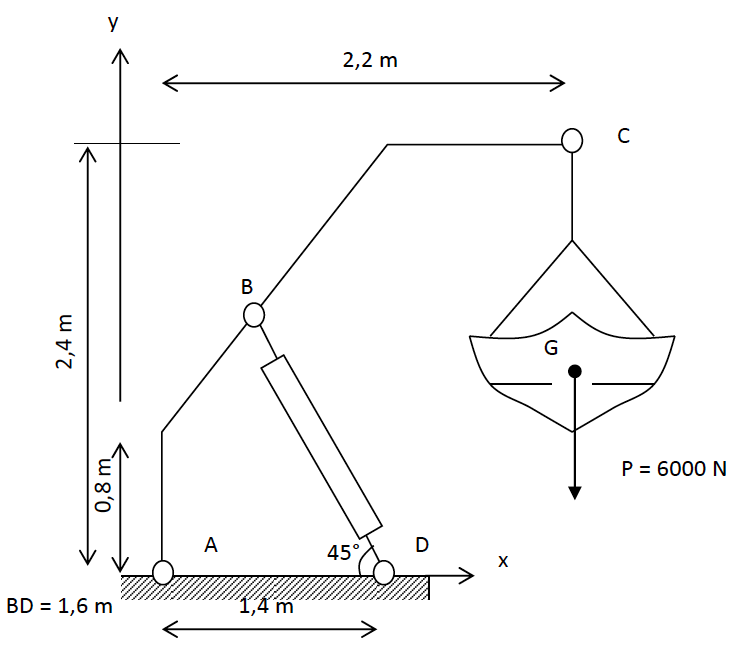
\includegraphics[scale=0.5]{png/grue.png}
\end{center}

Le système ci-dessus est en équilibre. Le bateau est maintenu par l'action du vérin hydraulique. Le problème sera supposé plan, et les liaisons pivot en $A$, $B$, $C$ et $D$ parfaites. L'action du poids sera négligée sauf
pour le bateau.

\subsubsection{Travail demandé}
\begin{enumerate}
\item Réaliser le graphe des liaisons de ce mécanisme.
\item Proposer une suite d'isolement permettant de calculer l’effort du vérin pour garder le bateau en équilibre. De manière graphique.
\item Déterminer analytiquement les actions mécaniques dans les liaisons en $A$, $B$, $C$ et $D$.
\end{enumerate}


\newpage

%--------------------------------------------

\exercice{Système de montage d'usinage}

On considère un mécanisme de serrage de pièce dans un montage d’usinage dont le dessin est donné ci-dessous.\\
Il est constitué de $3$ leviers $(1)$, $(2)$ et $(3)$.

\begin{itemize}
\item Le levier $(1)$ est lié au bâti $(5)$ par une liaison pivot d’axe $(B,\overrightarrow{z})$
\item Le levier $(3)$ est lié au bâti $(5)$ par une liaison pivot d’axe $(F,\overrightarrow{z})$
\item Le levier $(2)$ est lié aux leviers $(1)$ et $(3)$ par des liaisons pivots d’axes $(C,\overrightarrow{z})$ et $(E,\overrightarrow{z})$.
\end{itemize}

Toutes les liaisons sont supposées sans frottement et le poids des pièces est négligé devant les autres efforts.

\begin{center}
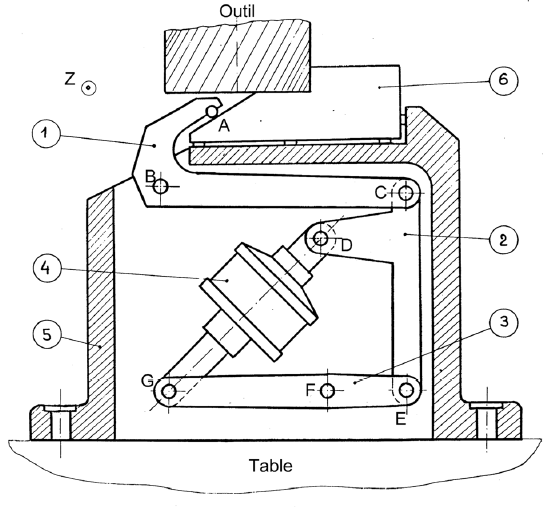
\includegraphics[scale=0.6]{png/montage.png}
\end{center}

\subsubsection{Travail demandé}
L’ensemble étant en équilibre par rapport à un repère galiléen, déterminer graphiquement les actions que doit exercer le vérin $(4)$ sur les deux leviers $(2)$ et $(3)$ pour que l’action du levier $(1)$ sur la pièce $(6)$ soit représentée par une force d’intensité 100 daN (le vérin $(4)$ est lié aux leviers $(2)$ et $(3)$ par des liaisons pivots sans frottement d’axes $(D,\overrightarrow{z})$ et $(G,\overrightarrow{z})$).

\newpage

%--------------------------------------------

\exercice{Poinçonneuse d’établi}

Le dessin ci-dessous représente une poinçonneuse d’établi. L’effort développé par le vérin est de $1000N$. Le coefficient de frottement aux contacts localisés en $M$ et $N$ est de $0,2$.

\begin{center}
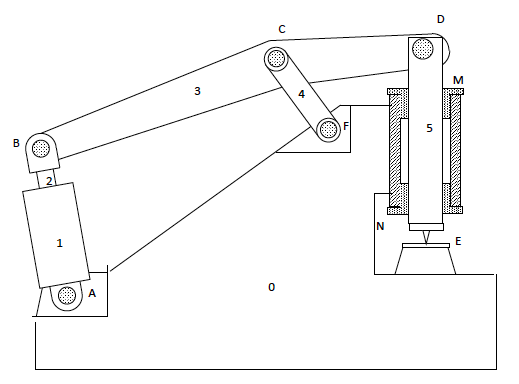
\includegraphics[scale=0.8]{png/poiconneuse.png}
\end{center}

\subsubsection{Travail demandé}
\begin{enumerate}
\item Déterminer graphiquement l’action du levier $(3)$ sur la broche $(5)$.\\
Un léger jeu entre $(5)$ et les coussinets en bronze oblige la broche à s’incliner légèrement dans son guidage.
\item Faire un bilan des actions mécaniques extérieures à la broche $(5)$ en donnant toutes les informations disponibles sur chacune. Faire le bilan des inconnues et montrer la faisabilité d’une résolution graphique.
\item Déterminer graphiquement toutes les actions mécaniques agissant sur $(5)$.
\end{enumerate}


\newpage

%--------------------------------------------

\exercice{Robot manipulateur}

Le robot manipulateur représenté \textit{figure $15$} par son schéma se compose :
\begin{itemize}
\item d'un socle $(1)$ pivotant autour de l'axe vertical $(O,\overrightarrow{y})$ par rapport à une base $(0)$, non représentée,
\item d'un bras mécanique constitué de deux parties :\\
$\bullet$ le \og bras \fg{} $(2)$, relié au socle par une articulation \og d'épaule \fg{},\\
$\bullet$ \og l'avant-bras \fg{} $(3)$, relié au bras $(2)$ par une articulation de "coude".
\end{itemize}
L'angle du bras $(2)$ par rapport à la verticale est commandé par un \og vérin d'épaule \fg{} $V_1$, l'angle de l'avant-bras $(3)$ par rapport à l'horizontale est commandé par un \og vérin de coude \fg{} $V_2$.\\
Les ensembles $(2)-(4)$ et $(3)-(5)$ constituent des parallélogrammes. A l'extrémité de l'avant-bras $(3)$, le moteur $(8)$ commande l'orientation du positionneur $(7)$ par rapport au poignet $(6)$.\\
Le robot étant immobilisé dans la configuration de la figure, la position des points particuliers dans le repère $R(O,\overrightarrow{x},\overrightarrow{y},\overrightarrow{z})$ est donnée, en millimètres, par :

\begin{description}
\item $\overrightarrow{OA}=-200\overrightarrow{x}$; $\overrightarrow{OB}=200\overrightarrow{x}$; $\overrightarrow{OC}=250\overrightarrow{x}+430\overrightarrow{y}$;
\item $\overrightarrow{OD}=360\overrightarrow{x}+630\overrightarrow{y}$; $\overrightarrow{OE}=610\overrightarrow{x}+1075\overrightarrow{y}$;
\item $\overrightarrow{OF}=610\overrightarrow{x}+1275\overrightarrow{y}$; $\overrightarrow{OH}=1050\overrightarrow{x}+825\overrightarrow{y}$;
\item $\overrightarrow{OI}=2080\overrightarrow{x}+420\overrightarrow{y}$; $\overrightarrow{OC}=2080\overrightarrow{x}+220\overrightarrow{y}$;
\end{description}

Le positionneur $(7)$ est immobilisé dans le plan de symétrie $(0,\overrightarrow{x},\overrightarrow{y})$ du robot et supporte la charge verticale $(K,\overrightarrow{P})$ telle que : $\overrightarrow{P}=-4000\overrightarrow{y}$ (en $daN$) et $\overrightarrow{OK}=2350\overrightarrow{x}$ (en millimètres).\\
On suppose les liaisons sans frottement et les pièces constituant le robot de poids négligeable devant $\overrightarrow{P}$.

\begin{center}
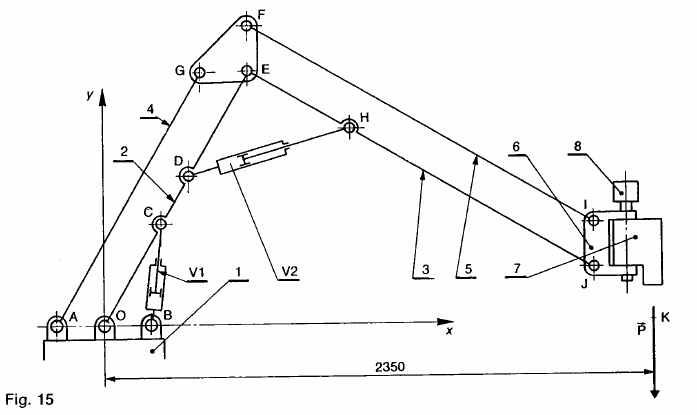
\includegraphics[scale=0.6]{png/manipulateur.png}
\end{center}

\subsubsection{Travail demandé}
Déterminer graphiquement et analytiquement les actions mécaniques exercées par les vérins $V_2$ et $V_2$ sur le bras.

\newpage


%----------------------------------------------------------------------------------------
%	Statique Analytique
%----------------------------------------------------------------------------------------

\section{Statique Analytique}

\exercice{Suspension d'un demi-train avant d'un véhicule}

La \textit{figure $11$} représente le schéma cinémamatique de la suspension d'un demi-train avant d'un véhicule Renault $4$.

\begin{center}
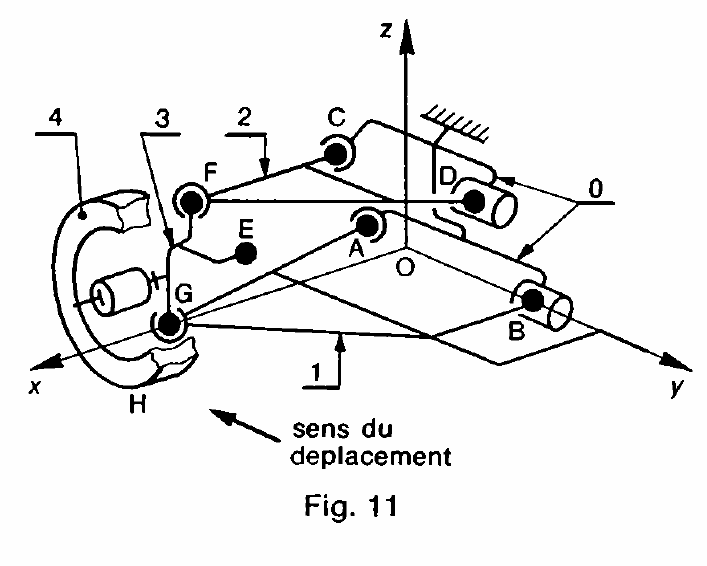
\includegraphics[scale=0.4]{png/suspension.png}
\end{center}

La suspension est constitée d'un triangle inférieur $(1)$ et d'un triangle supérieur, $(2)$, liés à la caisse par deux liaisons rotule de centre $A$ et $C$ et deux liaisons linéique annulaire d'axe $(B,\overrightarrow{y})$ et $(D,\overrightarrow{y})$ respectivement. Le porte moyeu $(3)$ a une liaison rotule de centre $F$ avec $(2)$ et une autre liaison rotule de centre $G$ avec $(1)$.\\
La biellette de direction, non représentée sur la figure, a une liaison rotule de centre $E$ avec $(3)$, et exerce sur $(3)$ une action mécanique représentée par la force $(E,F\overrightarrow{x})$. La barre de torsion d'axe $(O,\overrightarrow{y})$ exerce sur le triangle inférieur une action mécanique représentée par le couple de moment $C\overrightarrow{y})$.\\
La roue $(4)$ a une liaison pivot d'axe $(K,\overrightarrow{x})$ avec le porte moyeu $(3)$ (le véhicule se déplace en ligne droite).\\
On suppose que toutes les liaisons définis jusqu'à présent sont sans frottement et que les pièces constituant la suspension sont de masse nulle ainsi que la roue.\\
L'action mécanique de la route sur la roue est représentée par la force $(H,\overrightarrow{R})$ (le moment de roulement est négligé).\\
On pose : $N=\overrightarrow{z}.\overrightarrow{R}$. Soit $f$ le coefficient de frottement entre la roue et la route.\\
On donne, en millimètres, dans le repère $R(O,\overrightarrow{x},\overrightarrow{y},\overrightarrow{z})$ :
\begin{description}
\item $\overrightarrow{OA}=-100\overrightarrow{y}$; $\overrightarrow{OB}=200\overrightarrow{y}$; $\overrightarrow{OC}=50\overrightarrow{x}+400\overrightarrow{z}$;
\item $\overrightarrow{CD}=200\overrightarrow{y}$; $\overrightarrow{OG}=350\overrightarrow{x}$; $\overrightarrow{CF}=200\overrightarrow{x}$;
\item $\overrightarrow{FE}=150\overrightarrow{y}-150\overrightarrow{z}$; $\overrightarrow{GH}=50\overrightarrow{x}-150\overrightarrow{z}$.
\end{description}

\subsubsection{Travail demandé}
Le véhicule étant dans une phase de freinage brutal dans le sens de $-\overrightarrow{y}$, déterminer $F$ et $C$ ainsi que les actions mécanique dans les liaisons, sauf dans la liaison entre la roue et le porte moyeu. On se placera dans le cas où les roues avant sont à la limite du glissement par rapport à la route. On donne $N=440 daN$ et $f=0,9$.


\newpage

%--------------------------------------------

%\exercice{Train avant d'un véhicule}
%
%L’étude porte sur un mécanisme de suspension avant de véhicule automobile.\\
%\begin{center}
%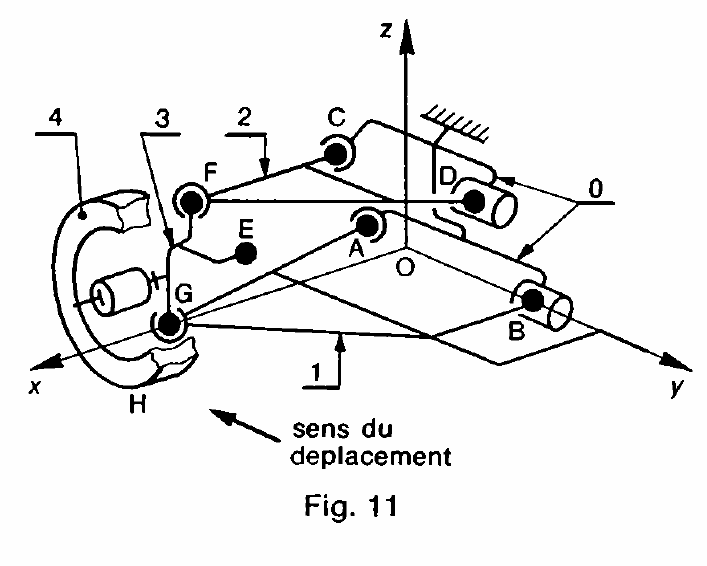
\includegraphics[scale=0.4]{png/suspension.png}
%\end{center}
%
%L’objectif de l’étude est de déterminer les efforts dans les différentes liaisons en vue de leur dimensionnement.
%
%\subsubsection{Hypothèses}
%\begin{itemize}
%\item Les liaisons sont parfaites
%\item Le véhicule est à l’arrêt
%\item Le poids des pièces est négligé devant les autres actions mécaniques
%\item L’action mécanique exercée par le sol sur l’ensemble 4+5+6 est modélisée par le torseur suivant :
%\begin{center}
%$T_{sol \longrightarrow 4+5+6} = \left\{
%\begin{array}{rcl}
%	 \overrightarrow{F_{sol \longrightarrow 4+5+6}=-F_x.\overrightarrow{x_0}+F_z.\overrightarrow{z_0}}\\
%	 \overrightarrow{0}
%\end{array}\right.$ en $L$
%\end{center}
%\item L’action mécanique exercée par la biellette de direction 10 sur l’ensemble 4+5+6 est modélisée par le torseur suivant :
%\begin{center}
%$T_{10 \longrightarrow 4+5+6} = \left\{
%\begin{array}{rcl}
%	 \overrightarrow{F_{10 \longrightarrow 4+5+6}=-F_y.\overrightarrow{y_0}\\
%	 \overrightarrow{0}
%\end{array}\right.$ en $L$
%\end{center}
%\end{itemize}
%
%\subsubsection{Données}
%Les centres des liaisons sont définis dans le repère $R_0=(B,\overrightarrow{x_0},\overrightarrow{y_0},\overrightarrow{z_0})$
%
%A compléter\dots
%
%\correction{ % Answer
%Correction \`a venir\dots
%}
%\newpage

%--------------------------------------------
